% !TeX root = main.tex

\documentclass[a4paper, oneside]{article}
% \usepackage[margin=2cm,bottom=4cm]{geometry}
\addtolength{\oddsidemargin}{-.25in}
\addtolength{\evensidemargin}{-.25in}
\addtolength{\textwidth}{1.in}

\usepackage{tsetsko-style}
\addbibresource{ref.bib}

\usepackage[section]{placeins}

\title{Final Project}
\date{\today}

\author{Tsvetelin Kostadinov}
\newcommand{\univname}{Sofia University "St. Kliment Ohridski"\\Faculty of mathematics and informatics}

\begin{document}
\begin{titlepage}
    \begin{center}
        \vspace*{-2.3cm}
        
\includegraphics[height=3cm]{resources/su_logo.png}

        \vspace*{.06\textheight}
        {\scshape\large \univname\par}\vspace{2.5cm}

        {\huge \bfseries{\thetitle}\par}\vspace{0.7cm}
        \textsc{\small in }\\[0.6cm]
        \textsc{\Large Numerical Methods and Algorithms}\\[0.5cm]\vspace{0.5cm}
        \textsc{\normalsize School year 2024/25}\\[0.6cm]\vspace{2.2cm}


        \begin{minipage}[t]{0.4\textwidth}
            \begin{flushleft} \large
                \emph{Supervisor:}\\[0.7cm]
                Prof. Ivan Dimov\\[0.7cm]
                Sofia\\[0.5cm]
                {\large 31.01.2025}
            \end{flushleft}
        \end{minipage}
        \begin{minipage}[t]{0.4\textwidth}
            \begin{flushright} \large
                \emph{Student:}\\[0.7cm]
                Tsvetelin Kostadinov Tsetskov\\[0.5cm]
                Faculty ID: 9MI3400529\\[0.5cm]
            \end{flushright}
        \end{minipage}

    \end{center}
\end{titlepage}

\begin{problem}\label{ex:1}
Show that the Lagrange form for $P_n$ can be rewritten as
\begin{equation}
    P_n(x) = w(x).\sum_{j=0}^n \frac{\beta_j}{x - x_j}f(x_j)
\end{equation}
where for any $n \in \N$, $j \in \N$ and $j \leq n$
\begin{align}
    P_n(x) = \sum_{j=0}^n l_j(x).f(x_j)                         \\
    l_j(x) = \prod_{k=0 \atop k \neq j} \frac{x-x_k}{x_j - x_k} \\
    w(x) = \prod_{k=0}^n (x - x_k)                              \\
    \beta_j = \frac{1}{\prod_{k=0 \atop k\neq j}^n (x_j - x_k)}
\end{align}
\end{problem}
\begin{solution}
    First, let us denote $f(x_i) = f_i$. We know that:
    \begin{align}
        P_n(x) = \sum_{j=0}^n l_j(x)f_j \\
        = \sum_{j=0}^n f_j \prod_{k=0 \atop k \neq j}^n \frac{x-x_k}{x_j - x_k}
    \end{align}
    for any $j$ we can rewrite $l_j$ in the form:
    \begin{align}
        l_j(x) = \prod_{k=0 \atop k \neq j}^n \frac{x-x_k}{x_j - x_k}                                                                              \\
        = \underbrace{\left( \prod_{k=0 \atop k \neq j}^n \frac{1}{x_j - x_k}\right)}_{=\beta_j} \left(\prod_{k=0 \atop k \neq j}^n x - x_k\right) \\
        = \beta_j \frac{1}{x - x_j} \prod_{k=0}^n x - x_k= \frac{\beta_j.w(x)}{x - x_j}
    \end{align}
    Substituting the result into $P_n$ we obtain the formulation:
    \begin{equation}
        P_n(x) = \sum_{j=0}^n \frac{f_j.\beta_j.w(x)}{x-x_j}
    \end{equation}
    Since $w(x)$ does not depend on the summation index, it can be extracted outside the sum:
    \begin{equation}
        P_n(x) = w(x) \sum_{j=0}^n \frac{\beta_j}{x-x_j}f_j
    \end{equation}
\end{solution}
\begin{problem}
Verify that
\begin{equation}
    1 = w(x).\sum_{j=0}^n \frac{\beta_j}{x - x_j}
\end{equation}
\end{problem}
\begin{solution}
    We can use the results from \exerciseref{ex:1} and consider $f(x) = 1$. We will use the fact that polynomials of degree $k \leq n$ overlap with $P_n$ (since we need $k+1$ points to fully describe the polynomial). So for $n \geq 0$ we have that $P_n(x) = 1$. Let's expand $P_n$:
    \begin{equation}
        1 = P_n(x) = w(x) \sum_{j=0}^n \frac{\beta_j}{x-x_j} \underbrace{f_j}_{=1} = w(x) \sum_{j=0}^n \frac{\beta_j}{x-x_j}
    \end{equation}
\end{solution}
\begin{problem}
A quadrature formula on the interval $[-1; 1]$ uses the quadrature points $x_0 = -\alpha$ and $x_1 = \alpha$, where $\alpha \in (0; -1]$:
\begin{equation}
    \int_{-1}^1 f(x) dx \approx w_0 f(-\alpha) + w_1 f(\alpha)
\end{equation}

The formula is required to be exact whenever $f$ is a polynomial of
degree 1 (i.e. $f(x) = a_0 + a_1 x$). Show that $w_0 = w_1 = 1$, independent of the value of $\alpha$.
\end{problem}
\begin{solution}
    Since the formula is required to be exact for a first-degree polynomial, we can solve the integral:
    \begin{align}
        \int_{-1}^1 f(x) dx = \int_{-1}^1 (a_0 + a_1 x) dx \\
        = (a_0 x + \frac{a_1}{2} x^2)\bigg\rvert_{-1}^1    \\
        = a_0 + \frac{a_1}{2} - (\frac{a_1}{2} - a_0) = 2.a_0
    \end{align}
    So now we can substitute $w_0 = w_1 = 1$ in the quadrature formula:
    \begin{align}
        w_0 f(-\alpha) + w_1 f(\alpha) = f(-\alpha) + f(\alpha) \\
        = a_0 - a_1.\alpha + a_0 + a_1.\alpha = 2.a_0
    \end{align}
    Indeed the formula is exact for polynomials of degree 1.
\end{solution}
\begin{problem}
Show that there is one particular value of $\alpha$ for which the formula is exact for all polynomials of degree 2. Find this $\alpha$.
\end{problem}
\begin{solution}
    Again we will solve the integral first:
    \begin{align}
        \int_{-1}^1 f(x) dx = \int_{-1}^1 (a_0 + a_1 x + a_2x^2) dx                 \\
        = (a_0 x + \frac{a_1}{2} x^2 + \frac{a_2}{3}x^3)\bigg\rvert_{-1}^1          \\
        = a_0 + \frac{a_1}{2} + \frac{a_2}{3} + a_0 - \frac{a_1}{2} + \frac{a_2}{3} \\
        = 2.a_0 + \frac{2}{3}a_2 \label{eq:quadrature-integral}
    \end{align}
    Let us assign $w_0 = w_1 = 1$ and evaluate the quadrature formula:
    \begin{align}
        w_0 f(-\alpha) + w_1 f(\alpha) = f(-\alpha) + f(\alpha)             \\
        = a_0 - a_1.\alpha + a_2.\alpha^2 + a_0 + a_1.\alpha + a_2.\alpha^2 \\
        = 2.a_0 + 2.a_2.\alpha^2 \label{eq:quadrature-formula}
    \end{align}
    It is evident that
    \begin{equation}
        \alpha = \sqrt{\frac{1}{3}}
    \end{equation}
    Equalizes the expressions in \eqref{eq:quadrature-integral} and \eqref{eq:quadrature-formula}
\end{solution}
\begin{problem}
The one-dimensional interpolation scheme can be applied to higher dimensions. Let the function $f(x, y) = e^x \sin y$ is given. We wish to construct a function of the form
\begin{equation}
    p(x, y) = c_0 + c_1x + c_2y + c_3xy + c_4x^2 + c_5y^2
\end{equation}
that interpolates $f(x, y)$ at $\vect{x_0, y_0}, \vect{x_1, y_1}, \vect{x_2, y_2}, \vect{x_3, y_3}, \vect{x_4, y_4}, \vect{x_5, y_5}$.
\end{problem}
\begin{solution}
    Again we denote $f_i = f(x_i, y_i)$

    We can setup the interpolation system as follows:
    \begin{equation}
        \begin{pmatrix}
            1 & x_0 & y_0 & x_0.y_0 & x_0^2 & y_0^2 \\
            1 & x_1 & y_1 & x_1.y_1 & x_1^2 & y_1^2 \\
            1 & x_2 & y_2 & x_2.y_2 & x_2^2 & y_2^2 \\
            1 & x_3 & y_3 & x_3.y_3 & x_3^2 & y_3^2 \\
            1 & x_4 & y_4 & x_4.y_4 & x_4^2 & y_4^2 \\
            1 & x_5 & y_5 & x_5.y_5 & x_5^2 & y_5^2
        \end{pmatrix}
        \begin{pmatrix}
            c_0 \\ c_1 \\ c_2 \\ c_3 \\ c_4 \\ c_5
        \end{pmatrix}
        =
        \begin{pmatrix}
            f_0 \\ f_1 \\ f_2 \\ f_3 \\ f_4 \\ f_5
        \end{pmatrix}
    \end{equation}
\end{solution}
\begin{problem}
    Write code to determine c when $f(x, y) = e^x \sin y$ and the $\vect{xi, yi}$ pairs take the values listed in the following table and report your value for $c$.
    \begin{table}[h]
        \centering
        \begin{tabular}{c|c c c c c c}
            \hline
            $j$ & 0 & 1 & 2 & 3 & 4 & 5 \\
            \hline
            $x_j$ & 0 & 0 & 1 & 1 & 2 & 2 \\
            $y_j$ & 0 & 2 & 0 & 2 & 1 & 3 \\
            \hline
        \end{tabular}
    \end{table}
\end{problem}
\begin{solution}
    Using the code at \figref{fig:exsiny-code}
    We obtain values for c:
    \begin{equation}
        c = \begin{pmatrix}
            0 \\ 
            -0.9491631051 \\
            5.059193000 \\
            0.7812146226 \\
            0.9491631051 \\
            -2.302272143
        \end{pmatrix}
    \end{equation}
\end{solution}
\begin{remark}
    A good observation for the function $f$ is that it is odd function in $y$ - this would simplify the calculation and make the matrix $A$ ''symmetric'' in a sense that we would have to calculate half as many points or use the available points for a better approximation and use an appropriate formula for odd functions
\end{remark}
\begin{problem}
    Plot your model function $p(x, y)$ over $x \in [-1; 3], y \in [-1; 3]$. Compare this plot to the similar plot for $f (x, y)$. Please submit plots of both $p(x, y)$ and $f(x, y)$.
\end{problem}
\begin{solution}
    The graphs can be found at \figref{fig:exsiny} and \figref{fig:approx-exsiny}
\end{solution}
\newpage
\begin{problem}
    Generate 11 data points, $t_k = \frac{(k-1)}{10}, y_k = \operatorname{erf}(t_k), k \in \set{1, \dots , 11}$.
    \begin{enumerate}
        \item Fit the data in a least squares sense with polynomials of degrees 1 through 10. Compare the fitted polynomial with $\operatorname{erf}(t)$ for values of $t_k$. How does the maximum error depend on the polynomial degree?
        \item Because $\operatorname{erf}(t)$ is an odd function of $t$, that is, $\operatorname{erf}(t) = -erf(-t)$, it is reasonable to fit the data by linear combination of odd powers of $t$:
        \begin{equation}
            \operatorname{erf}(t) \approx c_1 t + c_2 t^3 + \dots + c_n t^{2n-1}
        \end{equation}
        Again, see how the error at data points $t_k$ depends on $n$ using polynomials of degree up to 7.
    \end{enumerate}
\end{problem}
\begin{solution}
\begin{enumerate}
    \item Using the code in \figref{fig:erf-code} we obtain the graph in figure \figref{fig:max-error-vs-polinom-degree};
    \item Using the code in \figref{fig:erf-odd-code} we obtain a graph that does not look quite correct in a sense that the error is unpredictable with regards to the degree, however, we would expect it to be monotone decreasing. 
\end{enumerate}
\end{solution}
\begin{problem}
    A classical model in mathematical ecology is the Lotka-Volterra predator prey model. Consider a simple ecosystem consisting of rabbits that have an infinite supply of food and foxes that prey on the rabbits for their food. This is modeled by a pair of nonlinear, first-order differential equations:
    \begin{align}
        r(0) = r_0 \\
        \frac{dr}{dt} = 2r - \alpha r f \\
        f(0) = f_0 \\
        \frac{df}{dt} = -f + \alpha r f
    \end{align}
    where $t$ is time, $r(t)$ is the number of rabbits, $f(t)$ is the number of foxes, and $\alpha$ is a positive constant. If $\alpha = 0$, the two populations do not interact, the rabbits do what rabbits do best, and the foxes die off from starvation. If $\alpha > 0$, the foxes encounter the rabbits with a probability that is proportional to the product of their numbers. Such an encounter results in a decrease in the number of rabbits and (for less obvious reasons) an increase in the number of foxes. The solutions to this nonlinear system cannot be expressed in terms of other known functions; the equations must be solved numerically. It turns out that the solutions are always periodic, with a period that depends on the initial conditions. In other words, for any $r(0)$ and $f(0)$, there is a value $t = t_p$ when both populations return to their original values.

    \begin{enumerate}
        \item Using MATLAB compute the solution with $r_0 = 300, f_0 = 150$, and $\alpha = 0.01$. You should find that $t_p$ is close to 5. Make two plots, one of $r$ and $f$ as functions of $t$ and one a phase plane plot with $r$ as one axis and $f$ as the other.
        \item Compute and plot the solution with $r_0 = 15, f_0 = 22$, and $\alpha = 0.01$. You should find that $t_p$ is close to 6.62
        \item Compute and plot the solution with $r_0 = 102, f_0 = 198$, and $\alpha = 0.01$. Determine the period $t_p$ either by trial and error or with an event
        handler.
    \end{enumerate}
\end{problem}
\begin{solution}
    We will be using the code in \figref{fig:lotka-volterra} with modification in the initial conditions.
    \begin{enumerate}
        \item As we can see in \figref{fig:pop-vs-time-1} indeed the value of $t_p$ is close to 5. The phase diagram can be found at \figref{fig:phase-1}
        \item As we can see in \figref{fig:pop-vs-time-2} indeed the value of $t_p$ is close to 6.6. The phase diagram can be found at \figref{fig:phase-2}. Noteworthy is that at around $t=3.18$ we get really close to zero (evident from the graphs), however, the number is approx $1.3$ rabbits existing, thus the system can 'spring back'.
        \item The prepared graphics are \figref{fig:pop-vs-time-3} and \figref{fig:phase-3} (also experimented with longer simulation times in \figref{fig:pop-vs-time-3-long} and \figref{fig:phase-3-long}). We augment the code with \figref{fig:period} and determine that the period is around $4.38$ with a tendency to get lower and lower (evident from the graphs).
    \end{enumerate}
\end{solution}

\appendix
\section{Graphics}
\begin{figure}[h!]
    \centering
    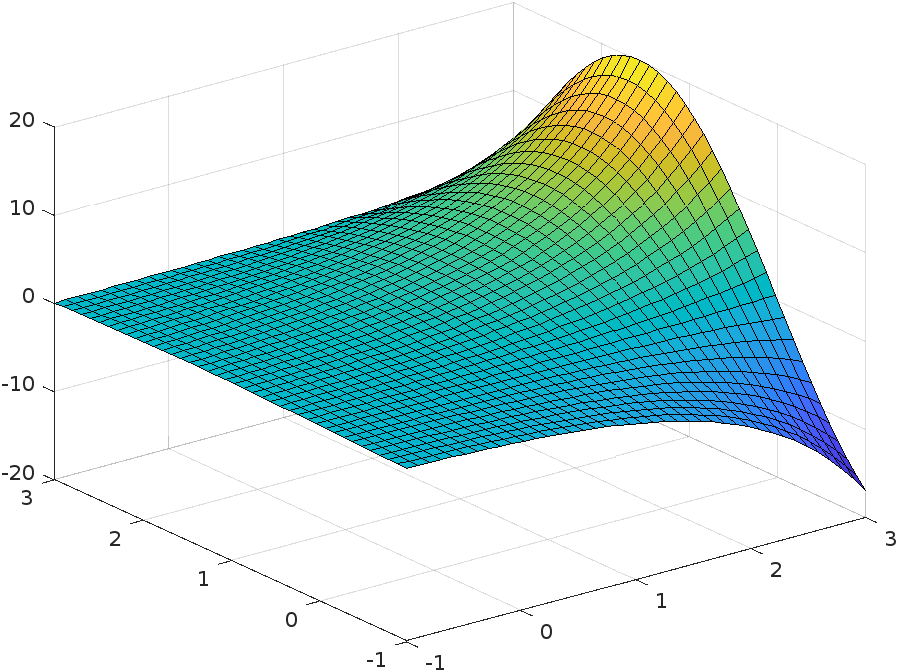
\includegraphics[width=\textwidth-9em]{resources/exsiny.png}
    \caption{Graph of $e^x.\sin y$}
    \label{fig:exsiny}
\end{figure}
\begin{figure}[h!]
    \centering
    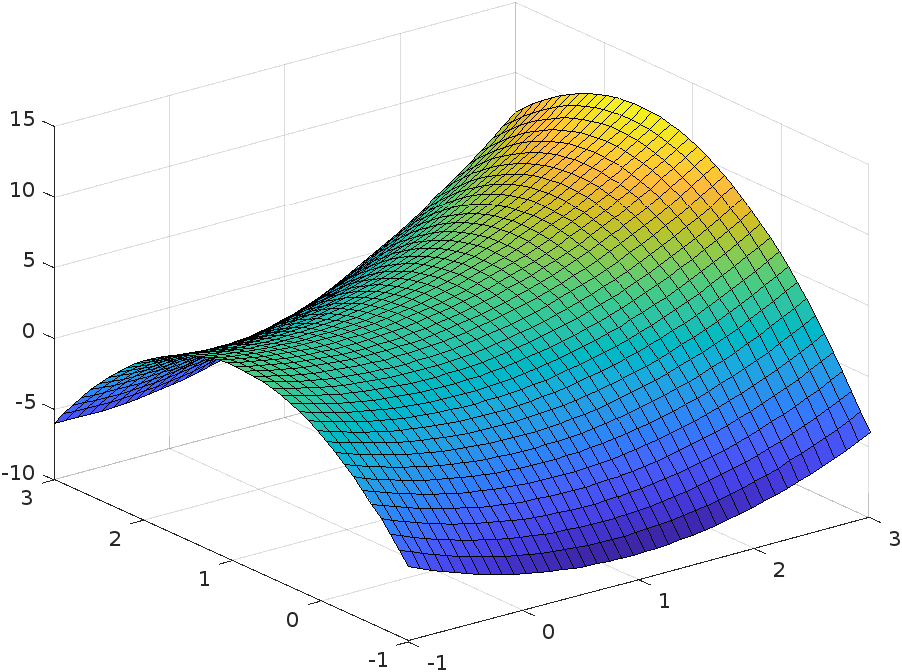
\includegraphics[width=\textwidth-9em]{resources/approx-exsiny.png}
    \caption{Graph of $p(x,y)$}
    \label{fig:approx-exsiny}
\end{figure}
\begin{figure}[h!]
    \centering
    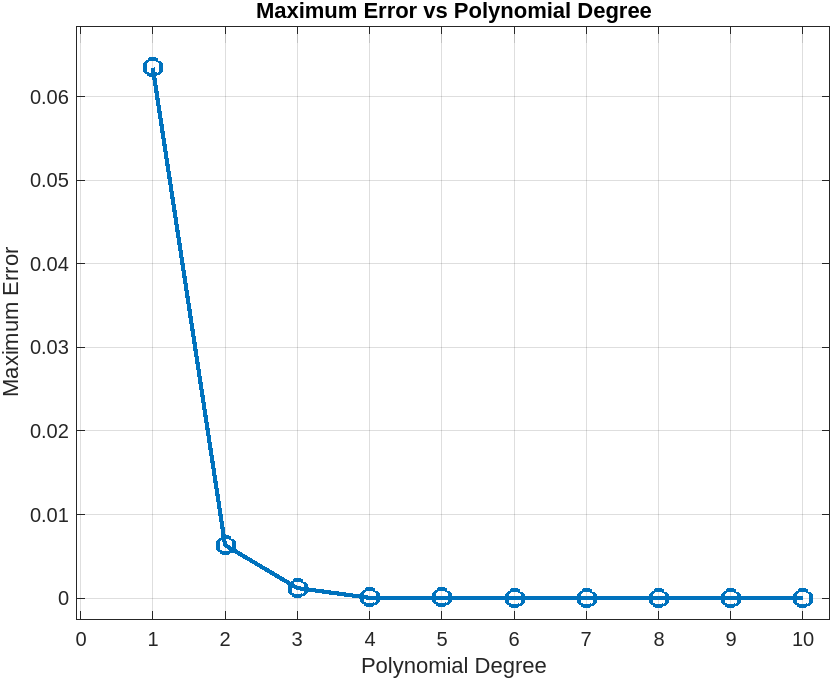
\includegraphics[width=\textwidth]{resources/max-error-vs-polinom-degree.png}
    \caption{Graph of the maximum error w.r.t. polinomial degree}
    \label{fig:max-error-vs-polinom-degree}
\end{figure}
\begin{figure}[h!]
    \centering
    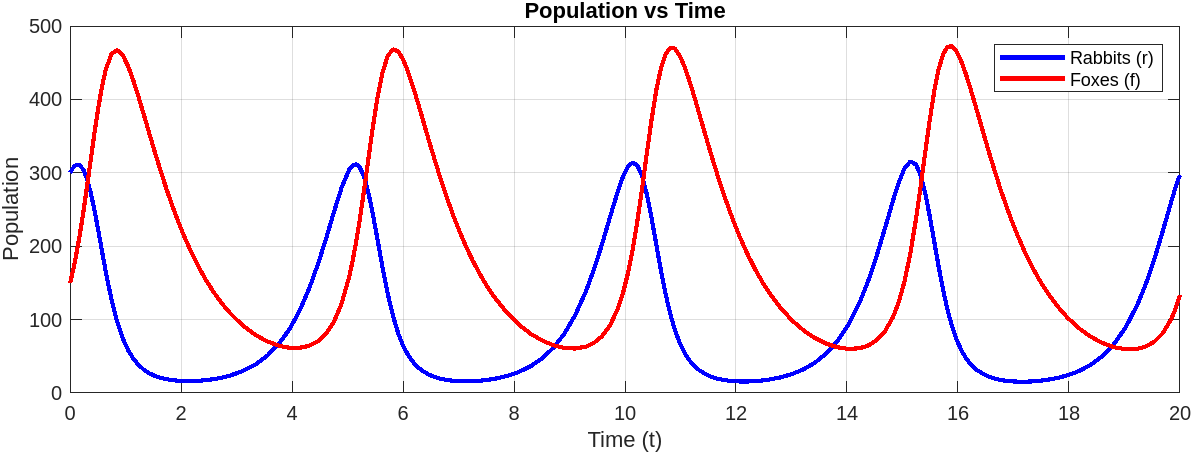
\includegraphics[width=\textwidth]{resources/pop-vs-time-1.png}
    \caption{Graph of populations vs. time for case 1}
    \label{fig:pop-vs-time-1}
\end{figure}
\begin{figure}[h!]
    \centering
    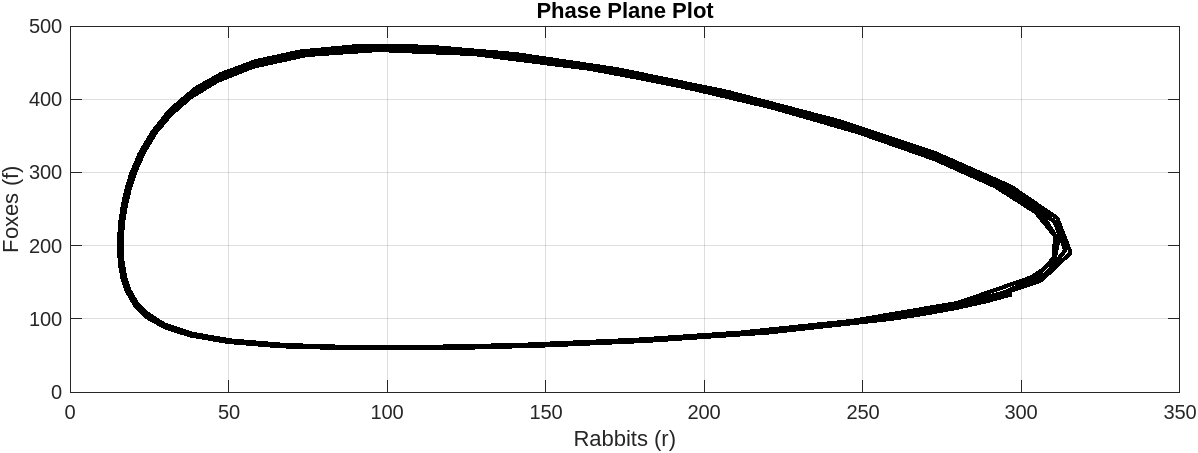
\includegraphics[width=\textwidth]{resources/phase-1.png}
    \caption{Phase graph for case 1}
    \label{fig:phase-1}
\end{figure}
\begin{figure}[h!]
    \centering
    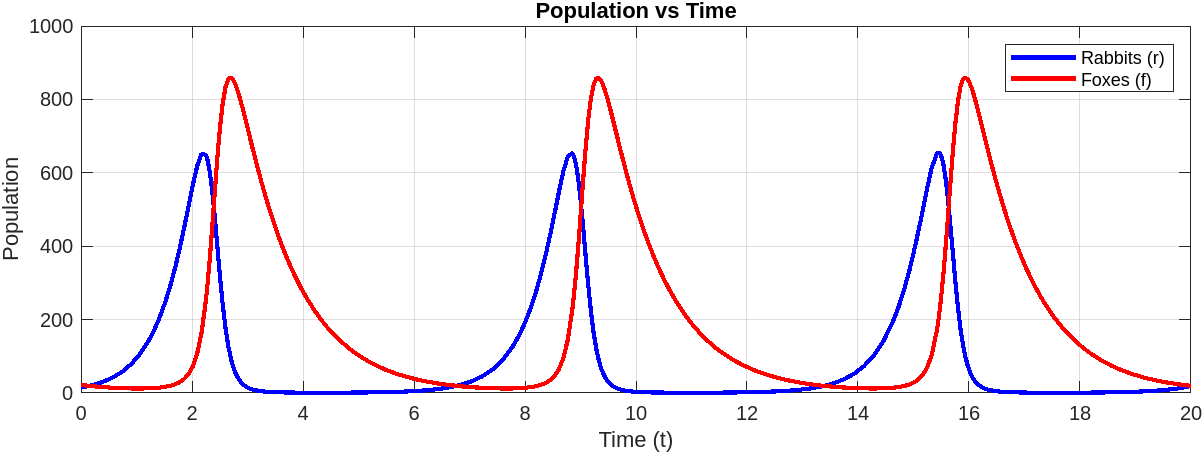
\includegraphics[width=\textwidth]{resources/pop-vs-time-2.png}
    \caption{Graph of populations vs. time for case 2}
    \label{fig:pop-vs-time-2}
\end{figure}
\begin{figure}[h!]
    \centering
    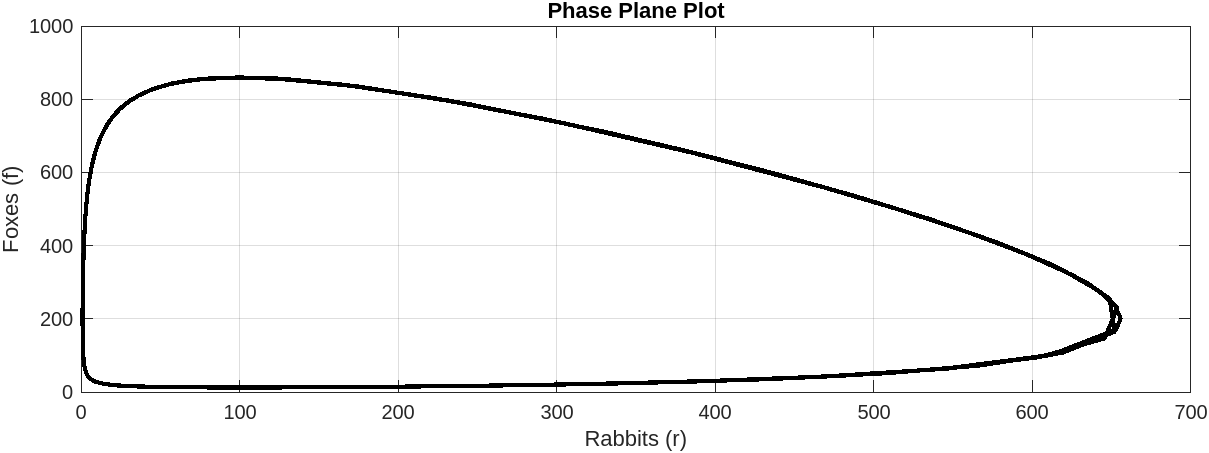
\includegraphics[width=\textwidth]{resources/phase-2.png}
    \caption{Phase graph for case 2}
    \label{fig:phase-2}
\end{figure}

\begin{figure}[h!]
    \centering
    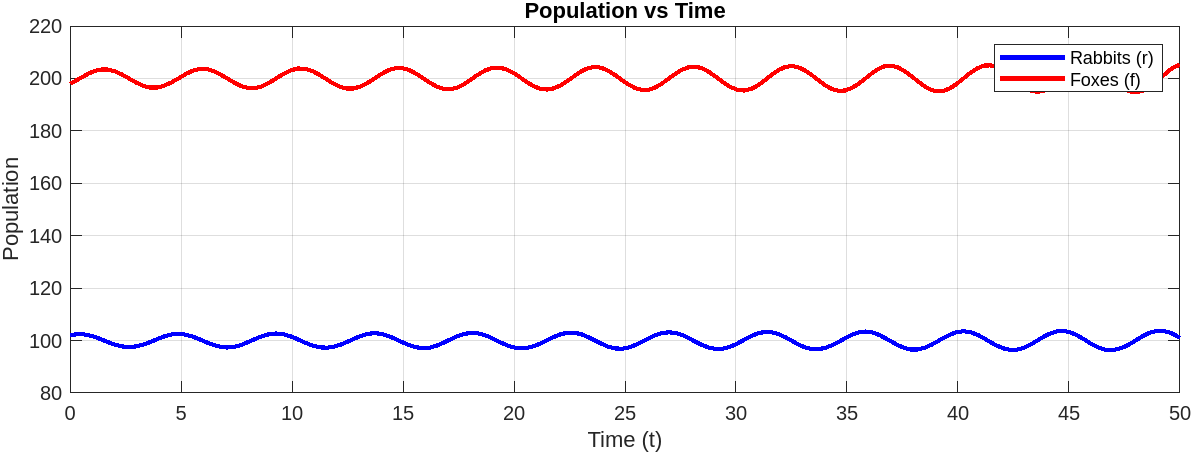
\includegraphics[width=\textwidth]{resources/pop-vs-time-3.png}
    \caption{Graph of populations vs. time for case 3}
    \label{fig:pop-vs-time-3}
\end{figure}
\begin{figure}[h!]
    \centering
    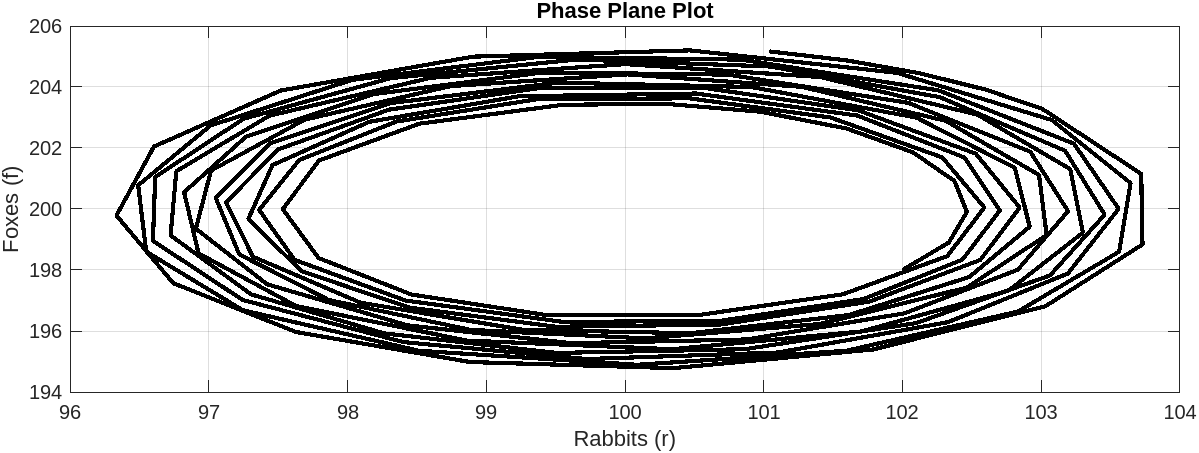
\includegraphics[width=\textwidth]{resources/phase-3.png}
    \caption{Phase graph for case 3}
    \label{fig:phase-3}
\end{figure}

\begin{figure}[h!]
    \centering
    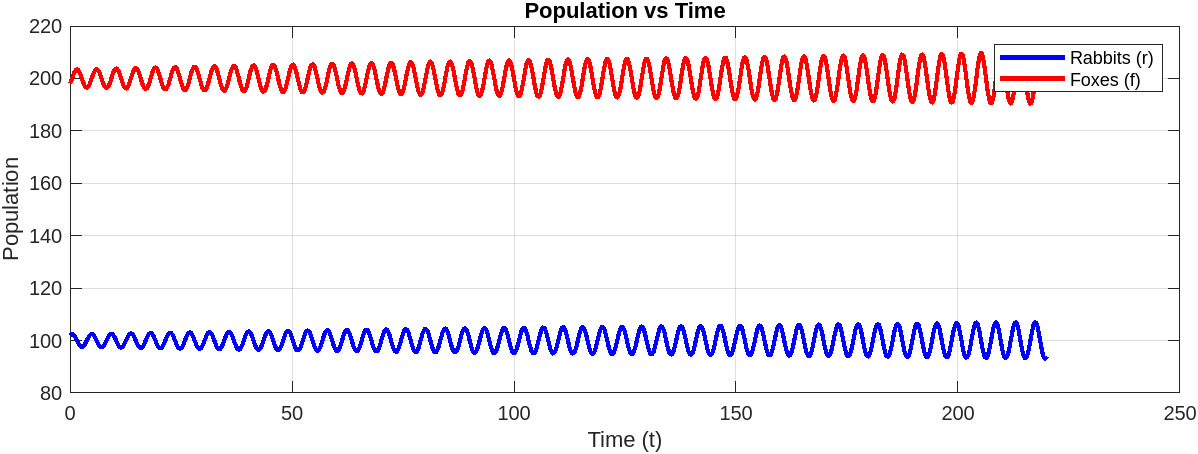
\includegraphics[width=\textwidth]{resources/pop-vs-time-3-long.png}
    \caption{Graph of populations vs. time for case 3 (longer simulation)}
    \label{fig:pop-vs-time-3-long}
\end{figure}
\begin{figure}[h!]
    \centering
    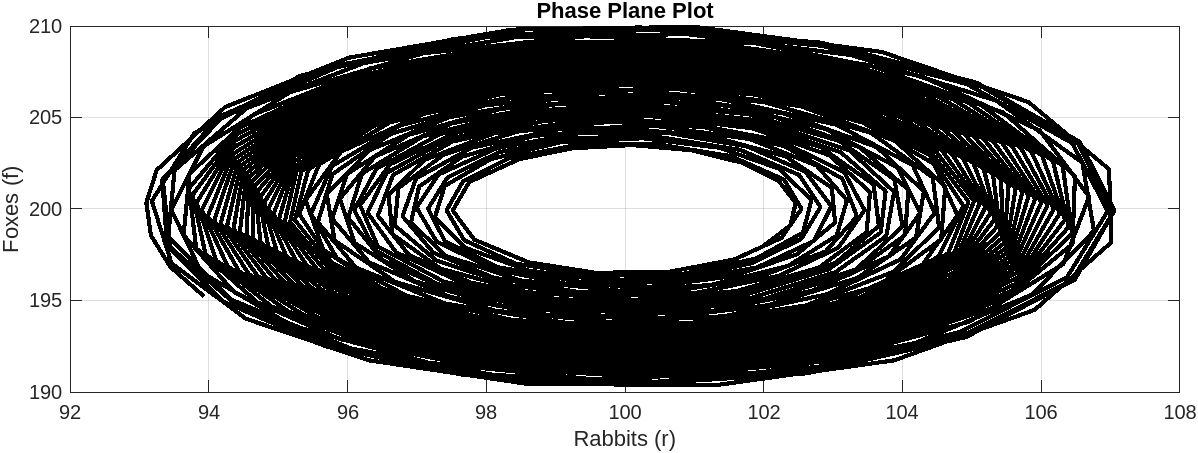
\includegraphics[width=\textwidth]{resources/phase-3-long.png}
    \caption{Phase graph for case 3 (longer simulation)}
    \label{fig:phase-3-long}
\end{figure}

\section{Code}
\begin{figure}[h!]
\begin{verbatim}
A = [1, 0, 0, 0, 0, 0;
     1, 0, 2, 0, 0, 4;
     1, 1, 0, 0, 1, 0;
     1, 1, 2, 2, 1, 4;
     1, 2, 1, 2, 4, 1;
     1, 2, 3, 6, 4, 9];

f = @(x, y) exp(x) * sin(y);

x = [0, 0, 1, 1, 2, 2];
y = [0, 2, 0, 2, 1, 3];

F = arrayfun(f, x, y).';

c = A \ F;

disp(c);

\end{verbatim}
\caption{MATLAB code to approximate coeffients}
\label{fig:exsiny-code}
\end{figure}

\begin{figure}[h!]
\begin{verbatim}
k = 1:11;
t = (k-1)/10;  % t_k = (k-1)/10
y = erf(t);    % y_k = erf(t_k)

degrees = 1:10;

max_errors = zeros(1, length(degrees));

for d = degrees
    p = polyfit(t, y, d);

    y_fitted = polyval(p, t);

    error = abs(y - y_fitted); 
    max_errors(d) = max(error);
end

figure;
plot(degrees, max_errors, '-o', 'LineWidth', 2, 'MarkerSize', 8);
xlabel('Polynomial Degree');
ylabel('Maximum Error');
title('Maximum Error vs Polynomial Degree');
grid on;
\end{verbatim}
\caption{MATLAB code to approximate $\operatorname{erf}$ with least-squares}
\label{fig:erf-code}
\end{figure}

\begin{figure}
    \begin{verbatim}
k = 1:11;
t = (k-1)/10;  % t_k = (k-1)/10
y = erf(t);    % y_k = erf(t_k)

max_degree = 7;

max_errors = zeros(1, (max_degree + 1) / 2);

for n = 1:max_degree
    X = [];
    for i = 1:n
        X = [X, t(1:n).^(2*i-1)];
    end
    
    c = X \ y;
    
    coeff_odd = fliplr(c);
    coeff = zeros(1, 2 *length(c));
    coeff(1:2:end) = coeff_odd;

    y_fitted = zeros(1, length(y));
    
    for k = 1:length(y_fitted)
        y_fitted(k) = polyval(coeff, t(k))

    error = abs(erf(t) - y_fitted);
    
    max_errors(n) = max(error);
end

figure;
plot(1:max_degree, max_errors, '-o', 'LineWidth', 2, 'MarkerSize', 8);
xlabel('Value of n');
ylabel('Maximum Error');
title('Maximum Error vs Polynomial Degree');
grid on;
    \end{verbatim}
    \caption{MATLAB code for approximating odd degree polynomial}
    \label{fig:erf-odd-code}
\end{figure}

\begin{figure}[h!]
    \begin{verbatim}
r0 = 300;  % Initial number of rabbits
f0 = 150;  % Initial number of foxes
alpha = 0.01;  % Predator-prey interaction constant

lotka_volterra = @(t, y) [
    2*y(1) - alpha*y(1)*y(2);  % dr/dt
    -y(2) + alpha*y(1)*y(2)   % df/dt
];

y0 = [r0; f0];

tspan = [0, 20];  % simulate from t = 0 to t = 20

[t, y] = ode45(lotka_volterra, tspan, y0);

r = y(:, 1);
f = y(:, 2);

figure;
subplot(2,1,1);
plot(t, r, 'b', 'LineWidth', 2);
hold on;
plot(t, f, 'r', 'LineWidth', 2); 
xlabel('Time (t)');
ylabel('Population');
legend('Rabbits (r)', 'Foxes (f)');
title('Population vs Time');
grid on;

subplot(2,1,2);
plot(r, f, 'k', 'LineWidth', 2);
xlabel('Rabbits (r)');
ylabel('Foxes (f)');
title('Phase Plane Plot');
grid on;
    \end{verbatim}
    \caption{MATLAB code for numerical solution of Lotka-Volterra model}
    \label{fig:lotka-volterra}
\end{figure}

\begin{figure}[h!]
    \begin{verbatim}
if length(crossings) >= 2
    tp = t(crossings(2)) - t(crossings(1));
    fprintf('Approximate period tp: %.2f\n', tp);
else
    fprintf('Could not determine period: Insufficient crossings detected.\n');
end
    \end{verbatim}
    \caption{Fragment for calculating the period}
    \label{fig:period}
\end{figure}


% \printbibliography
\end{document}